%%
%% This is file `sample-sigconf.tex',
%% generated with the docstrip utility.
%%
%% The original source files were:
%%
%% samples.dtx  (with options: `sigconf')
%% 
%% IMPORTANT NOTICE:
%% 
%% For the copyright see the source file.
%% 
%% Any modified versions of this file must be renamed
%% with new filenames distinct from sample-sigconf.tex.
%% 
%% For distribution of the original source see the terms
%% for copying and modification in the file samples.dtx.
%% 
%% This generated file may be distributed as long as the
%% original source files, as listed above, are part of the
%% same distribution. (The sources need not necessarily be
%% in the same archive or directory.)
%%
%% The first command in your LaTeX source must be the \documentclass command.
\documentclass[sigconf]{acmart}

%%
%% \BibTeX command to typeset BibTeX logo in the docs
\AtBeginDocument{%
  \providecommand\BibTeX{{%
    \normalfont B\kern-0.5em{\scshape i\kern-0.25em b}\kern-0.8em\TeX}}}

%% Rights management information.  This information is sent to you
%% when you complete the rights form.  These commands have SAMPLE
%% values in them; it is your responsibility as an author to replace
%% the commands and values with those provided to you when you
%% complete the rights form.

%%
%% Submission ID.
%% Use this when submitting an article to a sponsored event. You'll
%% receive a unique submission ID from the organizers
%% of the event, and this ID should be used as the parameter to this command.
%%\acmSubmissionID{123-A56-BU3}

%%
%% The majority of ACM publications use numbered citations and
%% references.  The command \citestyle{authoryear} switches to the
%% "author year" style.
%%
%% If you are preparing content for an event
%% sponsored by ACM SIGGRAPH, you must use the "author year" style of
%% citations and references.
%% Uncommenting
%% the next command will enable that style.
%%\citestyle{acmauthoryear}


\usepackage{array}
\newcommand{\head}[2]{\multicolumn{1}{>{\centering\arraybackslash}p{#1}}{\textbf{#2}}}

\usepackage{listings}



%%
%% end of the preamble, start of the body of the document source.
\begin{document}

%%
%% The "title" command has an optional parameter,
%% allowing the author to define a "short title" to be used in page headers.
\title{Meltdown: Reading Kernel Memory from User Space}

%%
%% The "author" command and its associated commands are used to define
%% the authors and their affiliations.
%% Of note is the shared affiliation of the first two authors, and the
%% "authornote" and "authornotemark" commands
%% used to denote shared contribution to the research.
\author{Enrik Doçi}
%%\authornote{Both authors contributed equally to this research.}
\email{enrik.doci@b-tu.de}
\orcid{1234-5678-9012}
\affiliation{%
  \institution{Brandenburg Technical University}
  \streetaddress{Universitatsstrasse 1}
  \city{Cottbus}
  \state{Germany}
  \postcode{03046}
}

%%
%% By default, the full list of authors will be used in the page
%% headers. Often, this list is too long, and will overlap
%% other information printed in the page headers. This command allows
%% the author to define a more concise list
%% of authors' names for this purpose.
\renewcommand{\shortauthors}{Enrik Doçi}

%%
%% The abstract is a short summary of the work to be presented in the
%% article.
\begin{abstract}
  A clear and well-documented \LaTeX\ document is presented as an
  article formatted for publication by ACM in a conference proceedings
  or journal publication. Based on the ``acmart'' document class, this
  article presents and explains many of the common variations, as well
  as many of the formatting elements an author may use in the
  preparation of the documentation of their work.
\end{abstract}

%%
%% The code below is generated by the tool at http://dl.acm.org/ccs.cfm.
%% Please copy and paste the code instead of the example below.
%%


%%
%% Keywords. The author(s) should pick words that accurately describe
%% the work being presented. Separate the keywords with commas.
\keywords{out-of-order execution, side-channel attack, transient instruction, + others}


%%
%% This command processes the author and affiliation and title
%% information and builds the first part of the formatted document.
\maketitle

\section{Introduction}

Content to be added later 
Aprox.  page



\section{Background}
Aprox. 2.5 pages.
To properly understand how Meltdown works, more specifically the steps to bypass memory isolation by taking advantage of out-of-order execution and further use timing differences in cache memory to create a covert channel, it is important to understand the purpose of each component used during this attack, and how they operate. This section is focused on the basics of memory hierarchy (caching and virtual memory) and an overview of CPU architecture to further understand out-of-order execution. 
\subsection{Memory Hierarchy}
\subsubsection{Caching}
The need for fast memory that could keep up with the CPU frequency is limited by the high cost per byte these high-performance memories come with.
To address this issue, extremely fast registers are placed inside the CPU, small but fast memory is assigned to the CPU, a slightly slower but random-based accessable memory is assigned to the running applications, and the secondary memory for storing data at rest. 

The memory close to the CPU, called a cache, takes advantage of {\itshape spatial locality} (data to be processed tend to be close to the data already being processed) and {\itshape temporal locality} (processed data tends to be requested multiple times during execution).

A typical architecture consists of 3 levels of caches, with two being private per core and the third one being shared. For efficiency, data is moved in {\itshape blocks} (or lines) which contain a fixed size of words. Placing the blocks in cache can be made via different schemes, such as {\itshape set associative} (each block has a pre-determined position in cache), {\itshape n-way set associative} (each block can be placed in one of n possible positions in cache) or {\itshape fully associative} (the block can be placed anywhere in cache).

The memory and speed of a typical modern desktop computer \cite{Hennessy:2017:CAS:3207796} tends to be as follows :

\begin{table}[h]
  \label{tab:freq}
  \begin{tabular}{p{0.66cm}|p{0.75cm}p{0.75cm}p{0.75cm}p{0.75cm}p{1cm}p{1cm}}
     & \textbf{CPU Reg.} & \textbf{L1 cache} & \textbf{L2 Cache} & \textbf{L3 Cache} & \textbf{Main Mem.} & \textbf{Secon. Mem.}\\
     \hline
    Size & 2000 Bytes & 64 KB & 256 KB & 8-32 MB & 8-64 GB & 256 GB - 2 TB\\
    \hline
    Speed & 300 ps & 1 ns & 3-10 ns & 10-20 ns & 50-100 ns & 50-100 $\mu$s\\
  %\bottomrule
\end{tabular}
\caption{Memory hierarchy for a Desktop Computer}
\end{table}

\subsubsection{Virtual Memory}
Each process runs within its own address space, so there is a need to share the limited main memory between all running processes. The method used to achieve this is through {\itshape virtual memory}; the physical memory is divided into blocks called pages, and allocated to any process in need for memory. The processor issues virtual memory addresses for memory operations, which are mapped to physical ones using page translation tables. The translation table is held inside a CPU register, and it is per-process only; the operating system updates them for every process being executed. 

In order for processes not to access the blocks of other processes, protection schemes have to apply. Translation tables have privilege checks that are enforced on access right type, such as readable, writable, executable and user accessible. Virtual address spaces are furthermore divided into user-space or kernel-space. The application currently being executed can have access to the user space, and only while running in privileged mode can the kernel space be accessed. Since the kernel needs to perform operations on user pages and not only on its own address space, it usually has the whole physical memory mapped. 

The OS updates the register with the process table of each process being executed on every context switch. This is a security mechanism that can only allow processes to reference their own virtual addresses since the page tables are implemented per process. 

To prevent attacks based on static addresses of data, non-executable stacks, canaries and address space layout randomization (ASLR) have been introduced \cite{}. Just like ASLR, KASLR (kernel address space layout randomization) is used to randomize on every boot the offset of the address space, making it harder to locate kernel objects on memory. Nonetheless, side-channel attacks can make it quite easy and feasible to derandomize KASLR \cite{}.

\subsection{CPU Architecture and out-of-order Execution}

The CPU architectures affected by the attack mentioned in this paper have all a microarchitecture that is pipelined, super-scalar, out-of-order and with speculative execution. This section will further explain each of these methods used to perform instruction-level parallelism (ILP).

{\itshape Pipelining} is a technique which allows multiple instructions to overlap during execution, each using different resources oft he processor. Standartization of instruction in execution phases such as fetch, decode, execute, memory access and write-back, which do not have hardware dependencies between them. 

{\itshape Superscalar} processors can execute more than one instruction during a clock cycle. This is not the same as multi-core processor, but rather having multiple execution resources inside the CPU, for example ALUs. 

{\itshape Speculative execution} means that the compiler or the processor tries to guess the outcome of an instruction, thus removing it as a dependency in the execution path of other instructions. Since out focus is the hardware architecture, the main speculative execution on a processor ist hat of branch predicition, explained below. 

{\itshape Out-of-order execution} makes it possible for instructions to continue execution the moment all the required resources are available, even when the previous one is blocked and waitting for other operations to be completed. This is not to be confused with speculative execution below; in out-of-order execution all the instructions are correctly executed and no assumptions are made. Still, all the execution results stay at an microarchitecture state till all prior instructions are commited. 

\begin{figure}[h]
  \centering
  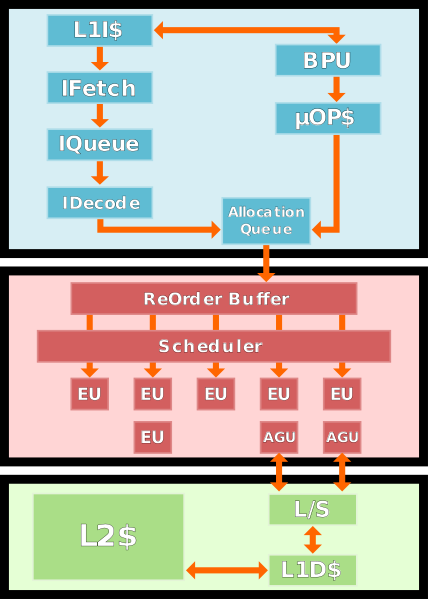
\includegraphics[width=\linewidth]{skylake_simple_diagram}
  \caption{Simplified design of a Skylake Core.}  
  \Description{The 1907 Franklin Model D roadster.}
\end{figure}

\footnote{ for detailed picture, choose skylake\_block\_diagram [Public domain maybe? check!!!], via (). }

The first step to achieve out-of-order execution is to solve data hazards (data dependencises from previous instructions), such as read-after-write, write-after-read and write-after-write (RAW, WAR, WAW). Normally, even in a pipelined datapath, the output from a previous instruction would be available only after the last phase, memory writeback. Tomasulo \cite{Cohen07} suggested the use of a unified reservation station that would make the outputs available the moment they were ready, and not having to wait for it to be stored and re-read using common data bus (CDB), that connects all execution units with each-other. 

In the front-end, instructions are decoded into micro-ops ($\mu$-ops), and are sent into the IDQ ($\mu$-op queue). Breaking every instruction into $\mu$-ops makes it possible for any procesor to execute commands without the need of modifying the instruction set. They are later sent to the back-end (execution engine) where the logic of out-of-order is implemented. They are later forwarded to the scheduler, which decides on which execution unit u-ops should be send depending on their specific task. 

BPU (Branch Prediction Unit) decides on branch instructions which block of code will be executed, before knowing for sure the correct flow of the execution. This prediction is usually a trade secret, and only the manufacterer knows the algorithm used, but the main ways to predict a path are : ---content here--- Instructions on the path that is going to be executed, start executing immediately as long as they don‘t have any dependencies. Upon realizing that the prediction was incorrect, the reorder buffer is rolled-back to a correct state (flushed) and the unified reservation station is re-initialized. This way, unauthorized instructions are executed and can change the microarchitectural state, but the change will not be reflected on the architecture state. 


\subsection{Cache Side-channel Attacks}
On his paper in 1994 contracted by the National Security agency, Sibert \cite{} states on the Intel 80x86 pprocessor architecture 
\begin{quote}
" caches present potential for covert timing channels ... cache hits and misses can be detected stricly from instruction timing "  
\end{quote}

To protect from these side channel attcks, protection mechanisms such as cache flushes and invalidation activity should be performed, which would cause a considerate drop on performance. To prevent this performance penalty, tradeoffs between performance, design complexity and security had to be made. While updating the ???

Cache side-channel attacks work by measuring time differencies introduce by caches. Hit times and miss penalties are measured as a constant number of cycles, making it easy to check if there was a hit or no, which memory answered the address reference and in what cache address was the block found. Combining the information from these parameters, quite high performance side-channel attacks can be performed.  

While at 2.3 Flush+Reload was used to transmit the data from the microarchitectural state to the attacker process, any other cache side-channel attack can be used. Such side-channel attacks are as below : \cite{8686667}

\subsubsection{Evict+Time}

In this attack, the attacker evicts certain cache sets and then measures the execution time of the victim’s code to determine whether the victim used a memory location that maps to the
evicted cache sets. While EVICT + TIME attacks provide a lower bandwidth than PRIME + PROBE attacks [33], they are effective in high-noise environments such as JavaScript [12].

\subsubsection{Prime+Probe}

PRIME + PROBE attack, the attacker builds an eviction set of memory addresses to fill a specific cache set. By repeatedly measuring the time it takes to refill the cache
set, the attacker can monitor memory accesses to that cache set. Furthermore, as part of the memory address determines the cache set to which the address maps, the attacker can infer information about the memory address used to access the cache set. Thus, by monitoring different cache sets, an attacker can determine, for example, which part of a look-up table was used by a victim process. While PRIME + PROBE originally targeted the L1 cache [33] to monitor accesses from the same processor core or another hardware thread, the inclusive nature of
the LLC in modern Intel processors has led recent work to target the LLC [21, 23, 31], enabling PRIME + PROBE in cross-core and cross-VM setups.
PRIME + ABORT [8] is a variant of PRIME + PROBE that leverages Intel’s Transaction Synchronization Extensions (TSX). Intel TSX introduces support for hardware transactions, where the L1 and L3 caches are used as write and read sets, respectively, to keep track of addresses accessed within the transaction. PRIME + ABORT monitors accesses to a single cache set by filling the cache set during a transaction as any additional accesses to same cache set causes the transaction to abort.

\subsubsection{Flush+Reload}
Flush+Reload\cite{Knuth97} is a side-channel attack technique with minimal noise induction, that has been used to implement in practice Meltdown attacks. This attack exploits a weakness on Intel X86 processors, where access to memory lines in shared pages can be monitored, and used to leak informations from processes. It targets the L3 cache, thus the attack can be performed even on other execution cores. 


To reduce the memory footprint, running processes often share identical memory pages. Shared libraries is a prime example of sharing (code) pages. Another example is memory deduplication [32], where an active process searches for pages with identical contents to coalesce them. While there are hardware mechanisms in place to ensure isolation between processes by enforcing read-only or copy-on-write semantics for shared pages, the existence of shared caches results in an exploitable side-channel for such pages. Gullasch et al. [17] use the CLFLUSH instruction to evict targets to monitor from the cache. By measuring the time to reload them the attacker determines whether the victim has accessed them—a class of attacks called FLUSH + RELOAD. Further, Yarom and Falkner [42] observe that CLFLUSH evicts a memory line from all the cache levels, including the lastlevel cache (LLC) which is inclusive of the lower cache levels and shared between all processor cores, thus enabling an attacker to monitor a victim from another processor core. In addition, the FLUSH + RELOAD attack allows for cross-VM attacks.
A variant of FLUSH + RELOAD, FLUSH + FLUSH [16] builds upon the observation that CLFLUSH aborts early in case of a cache miss, leading to a side channel. As the FLUSH + FLUSH attack relies only on the CLFLUSH and performs no memory accesses, it is a stealthier alternative to FLUSH + RELOAD.

\begin{figure}[h]
  \centering
  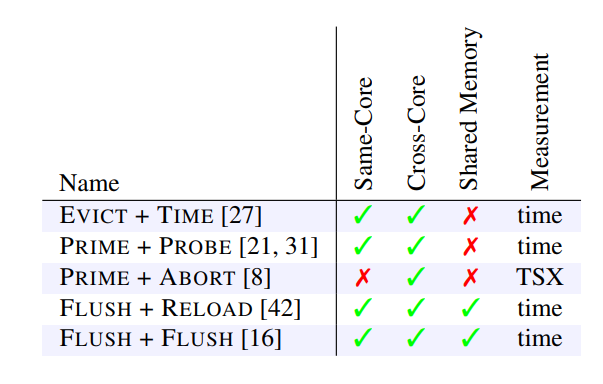
\includegraphics[width=\linewidth]{side-channel}
  \caption{Simplified design of a Skylake Core.}  
  \Description{The 1907 Franklin Model D roadster.}
\end{figure}

\section{Meltdown}
Aprox. 2 pages.
The main idea of meltdown is to throw an unhandled exception, which will cause the operating system to take control of the execution flow and handle the exeption. This means that the control flow will execute in kernel mode. Till now, nothing out of the ordinary happens, but due to out-of-order execution, the next few instructions being executed, now will run on kernel space and not user space. These instructions will not be retired, thus not saving the microarchitectural changes and the results of the executed instructions.

To have access to kernel data, a simple move instruction can be performed, causing the byte referenced in the memory to be fetched and stored in a register, and also cached . While not much can be done to retrieve the data from te register since it will not be commited, the cached values will continue to stay on.

The atack consists of two steps; first to make the CPU execute so-called transient instructions, instructions that should logically not be executed and whose result will not be stored. Transient instructions get executed all the time in order to minimize latency and improve the overall performance of the processor. 
The second step is to built a covert channel to be able to transfer the values from a microarchitectural state to an architectural one. 

\subsection{Executing Transient Instruction}
When the exeption is raised after requesting pages the user is not allowed to, such as kernel pages or pages from the address space of other processes, two approaches are prpposed, to either handle the exeption or supress it. 

When using exeption handling, transient instructions are executed in the child process. The recovery of the microarchitectural state can be performed by the parent process using one of the methods mentioned previously. 
To do so, the attacker needs to modify the running application, so that when accessing the memory, the child process is terminated, and not the main one. 
To step up the performance of the attack, by installing a signal handler, the attacker can have control over the segmentation fault exeption. This way the attack doesnt need to keep creating and terminating child processes, but perform the attack under one process. 

Another method to execute transient instructions would be by using exeption supression. This is achieved by using transactional memory; grouping all the memory accesses together into one operation and if an error happens, the architectural satte is rolled back to the previous one. After resetting the state, there will be no exeption raised at all, and the micro-state can be observed via a covert channel. 

Another method to suppress exeptions would be following a spectre \cite{} like approach by using speculative execution. In speculative execution, instructions are executed before figuring out whether the branch should be taken or not, using branch prediction. By putting the instructions that perform the reading of protected memory after the conditional branch instructions, and performing some training on the branch prediction algorithm, the instructions will be executed, thus reading kernel memory or that of other processes. In this case as well, an exeption will not be thrown since the microarchitectural state will be flushed after the CPU figures the branch prediction was incorrect. 

\subsection{Saving the Microarchitectural State}

The execution of transient instructions happens all the time, and is not a security violation in the proccessor design or implementation, even when the attacker can inject custom intructions. 
The out-of-order execution becomes a threat only when the microarchitectural state can be transfered into an architectural state

The following machine code instructions can be easily used to give the basic concept of the attack, while removing the complexity of a real world example. 
\begin{lstlisting}[caption = Some random text caption goes here]
   ; rcx = kernel address
   ; rbx = probe array
   xor rax, rax
   retry:
   mov al, byte [rcx]
   shl rax, 0xc
   jz retry
   mov rbx, qword [rbx + rax]
\end{lstlisting}

The move instruction reads the byte at address where the register rcx points to, and copies the value to register al. Since this address falls under the kernel space, an exeption will be thrown, and the execution will jump to the exception handler. In this case the exception will be a page fault, and the operating system will discard all the instruction executed during the out-of-order execution. 

\subsection{Performing the attack}

In order to perform a succsesful attack and extract the data from protected memory, first of all an address from the main memory that the attacker wants to be read should be referenced as a virtual address. As shown on the code above, on line 3 we try to read a byte from a kernel address space. As explained on Section 2, the instruction is fetched, decoded, allocated and forwarded to the reorder buffer. During this time, even the rest of the instructions are already decoded into uops, and are forwarded to the reservation unit waiting for an ALU to be freed and execute them. 

After being executed, under a normal execution, uops will retire in order. During the retirement, if there are any interruptions or exceptions, they are handled first. In our case, the MOV instruction will raise and exception, which will cause the pipelinne to be flushed and the results of the instructions executed out-of-orded to be lost. If the attacker manages to transmit the state after the execution of the uops before the exception is raised, the secret values from the choosen memory address can be successfuly retrieved. To transmit the value which was read, we use the transient instruction sequence following the MOV instruction, which will be executed out-of-order. These instructions should be short and quick to transmit before the previous instruction is retired, later causing an exception and flushing the datapath. Since the transmission from a microarchitectural state to an architectural one cant be done directly and explicitly, the transient instructions will be used to create a covert channel.

As discussed on section 2, multiple cache side-channel attacks can be used to transmit, but since the environment is low-noise and it requires a fast channel, the best choice would be Flush+Reload. To perform this, a probe array is allocated from the main memory and it needs to be completely uncached. Only one of the blocks will be cached, whose referenced address will be the data read .

In the Meltdown code above, the data read is multiplied by the cache size (0xC, 2power12), in this case 4KB. This is done to make sure that array accesses are far from each other, so they have a large spatial distance and can't be prefetched in group together in the same cache. 

The next line makes sure to reduce the noise-bias towards the value 0, which will be explained later. Basically it makes sure that if the value read is 0, it will retry reading it. Lastly the calculated value after the multiplication is added to the base of the probe array. We now have the target address, which will be read and cached in L1 and at the same time L3. At this point it is clear how a transient instruction sequence managed to change the state of the caches, making it possible to detect the change from any of the cores. 

Lastly, the attacker should only recieve the value through the recieving end of the covert channel built on the previous step. As mentioned previously, the index of the cached page is determined by the secret value read only. To get this value, the probe array should be iterated and the timing differencies are measured. It is clear which line was cached, due to the hit time being low. 

Till now, we only explained how we could read the value of one memory address. By iterating the procedure explained above, the attacker can dump the complet memory. To do so, exception handling or exception suppressing as mentioned more in detail the previous paragraph, should be used. 
Since every popular OS maps the whole physical memory into the kernel address space of every process, Meltdown can be used to completely read the physical memory as well. 


\section{Proof of Concept}

Text here. Aprox. 1.5 Pages.

\subsection{Meltdown-type Attacks}
Different Meltdown variations were implemented, making it possible to exploit different exception types and even exploit AMD CPUs using delayed exeption handling. 

In the aftermath of the Meltdown and Spectre attacks being published, on their paper evaluating trnasient execution attacks and defenses, Canella et al. \cite{Canella2018ASE} categorise Meltdown attacks as follows :

\subsubsection{Meltdown-US (Supervisor-only Bypass)}
 - This is the original implemenatation of the Meltdown attack but using the "user/supervisor" page table implemented in modern CPUs used to denote OS kernel virtual memory pages. 
 Features such as exception handling \cite{}, Intel TSX \cite{} and exception suppressing in another transient execution \cite{} can greatly improve the attack bandwidth. 

\subsubsection{Meltdown-P (Virtual Translation Bypass)}

A new Meltdown like attack proposed by Van Bulck et al. \cite{} targets the Intel SGX \cite{} technology, which makes plan Meltdown unusable since it doest raise a Page Fault exception, but replaces the unauthorized memory values with dummy values. The attacker in this case needs to clear the "present" flag from the TLB entry, causing page faults to be raised for further memory accessses. Further information on why this happens was published by Intel \cite{} .

This attack can only be performed agains L1 cache, but the implication is that foreshadowing can bypass isolations provided by the OS or by the hypervisor. Foreshadow-NG \cite{} variant for VMM makes it possible for a virtualmachine to read the host data from the L1 cache and extract it. 

\subsubsection{Meltdown-GP (System Register Bypass)}

Meltdown GP \cite{} was discovered by ARM \cite{}, but it can be performed even for Intel CPUs \cite{}. This variant of Meltdown only allows reading system registers. While the idea is the same as plain Meltdown, the request to read data is made towards privileged system registers, which will cause a general protection fault. The transient instructions can still continue working on those values and leak the results via a microarchitectural covert channel. 


\subsubsection{Meltdown-NM (FPU Register Bypass)}

This variant of Meltdown takes dvantage of the lazy state switch to cause a device-not-available exeption. Lazy state switch is a performance-wise solution OSes perform during contex switches. Saving all registers on every contex switch, espacially the large ones such as SIMD or floating point unit (FPU), would slow the switch, thus these registers are not saved and moved back, but rather just marked as "not available" and if a FPU instruction is issued, the exeption is thrown. 

A proof of work is given by Steclina and Precher \cite{} with similar steps as Meltdown. After the victim loads data in FPU registers, an attacker can switch in and the CPU will mark the FPU as not available. Now the attacker can issue FPU instructions that will generate the device-not-available exeption and at the mean time transient instructions are executed 

\subsubsection{ Meltdown-RW (Read-only Bypass)}

Meltdows-RW is a variant of the attack that can bypass access rights within the same privilege level, and not like the other approaches where the information is stolen between different privilege levels. Kiriansky and Waldspurger \cite{} based this variant on the fact that transient instructions don't respect the read and write attributes on a page-table. This allows to bypass software isolation and sandboxing methods that use hardware check of read-write memory.  

\subsubsection{Meltdown-PK (Protection Key Bypass)}

Used to defeat protection schemes offered by memory-protection keys for user space (PKU) mechanism implemented by Intel Skylake server CPUs \cite{}. Intel \cite{} states that no software solution can be implemented to offer protection from this Metdown flavor, but using address space isolation, this attack can be mitigated. 

\subsubsection{ Meltdown-BR (Bounds Check Bypass)}



\subsubsection{Residual Meltdown (Negative Results)}

 

\section{Countermeasures and Mitigation}

The countermeasures to protect from Meltdown would require modifications of the hardware itself and the datapath. While this would be possible only on further chips produced, in order to protect the current machines till they slowly roll out of service microcode updates should be issued, and other protection methods such as KAISER \cite{} are suggested to protect from side-channel attcks. 

\subsection{Hardware and Microcode Updates}

The first thing that comes to mind would be to completely disable out-of-order execution, but this is not a solution performance-wise since it would completely 
Another naive solution would be to wait for permission checks to be performed before the execution of register fetching. This would as well result in a big performance drop and is not a viable solution as well. 

The most solid option would be to split the user and kernel space. By realocating the kernel space in the upper part of the memory and the user space on the lower one, it would be quite easy for the fetch to realize whether the memory address would violate any privilege level just by checking the virtual address range, while at the same time causing a really minimal performance drop. While this would prevent Meltdown-like attacks mentioned at the next section, it would not offer protection agains Spectre \cite{} and other similar attacks. Thus kernel modification are suggested to protect existing architectures. 

\subsection{KAISER and KPTI}
The most obvious countermeasure would be to map the kernel space in a complete different location as the user space. This would prevent all the side-chanel attacks on the current KASLR implementation of randomizing the kernel address space. 
A suggestion is given by Gruss et al. in their proposed paper KAISER \cite{} (Kernel Address Isolation to have Side-channels Efficiently Removed), later called KPTI (Kernel Page Table Isolation) . 

Previously it was believed that KASLR vulnerabilities could leak just the location of memory mapping \cite{}, but not the contents of  kernel memory as well, as Meltdown attack manages to do. This was the main protection goal of KAISER  which by doing so, protects against Meltdown based attacks. 

KPTI was believed to induce only a 0.28\% performance drop when first published \cite{}, 


\section{Related Works}
Aprox. 1 page.
Exploitation can be observed during multiple steps of ILP. In the front-end this can happen during speculation via branch prediction (BPU), albeit difficult to exploit in the wild due to the mechanics of dynamic branch prediction not being publicly known. Exploitations can further be performed during dynamic scheduling (BPU \& IFU) and speculative execution (IDQ).

In the back-end exploitations can be observed during the register renaming (allocate/rename/retire unit), superscalar and out-of-order (scheduler) and in-order commit (retirement).

\subsection{Spectre}

While Meltdown makes use of the out-of-order execution to read and leak kernel memory that under normal execution they should not have, Spectre uses speculative execution property of branch prediction (conditional and indirect branches) to read arbitrary memory. Before BPU realizes the branch was wrongly predicted, some instructions are already speculatively executed, and through a side channel the confidential information is sent from a microarchitectural state to an architectural one. 

Unlike Meltdown, Spectre works on a wide range of processors, including most ARM and AMD models and not just Intel and some ARM. Also, KAISER mechanism used to mitigate Meltdown, doesn't protect against Spectre. 

\subsection{ZombieLoad}

ZombieLoad is another Meltdown-like attack that benefits from fault-driven transient instruction execution. This exploitation is performed on the fill-buffer using faulty Load instructions that have to be re-issued internally but don't become architecturaly visible. The values accessed by these Load instructions are those of recent registers belonging to previous memory operations from the current or a sibling hyperthread, unlike Meltdown that has to use explicit address-based selectors. Protection against ZombieLoad can be achived only by disabling hyperthreading. 


\newpage
%%
%% The next two lines define the bibliography style to be used, and
%% the bibliography file.
\bibliographystyle{ACM-Reference-Format}
\bibliography{sample-base}

%%
%% If your work has an appendix, this is the place to put it.
\appendix

\end{document}
\endinput
%%
%% End of file `sample-sigconf.tex'.
